We organize our results into four subsections, with each subsection focusing on experiments using one data set.

\subsection{Cloverleaf3D Simulation}
\label{sec:clover}

\textbf{Weak Scaling Study.} We considered 17 configurations of the Cloverleaf3D simulation in our weak scaling \textbf{Workflow1} study. 
%
Our experiment configurations span $81^{3}$ cells across 2 MPI ranks on 1 CN to $812^{3}$ cells across 2048 MPI ranks on 512 CNs, with each MPI rank operating on an approximately $64^{3}$ grid.
%
In each case, one GPU is assigned to every MPI rank, and we vary the number of ranks per CN.
%
For the number of MPI ranks on each CN, we consider 1 test using 2 ranks, 10 tests using 4 ranks, and 6 tests using 6 ranks.
%
For each run, we terminated the simulation after 500 cycles.
%
Given the variation in grid size, each test reaches a different stage of the simulation.
%
As the simulation grid size increases, the step size used by the simulation decreases.
%
We believe this is an acceptable assumption for most simulation codes.
%
With respect to parameterization of the Lagrangian flow map computation, we use a storage interval of 25 cycles and a data reduction of 1:8 ($\approx32,768$ particles seeded per MPI rank) for every test.

Figure~\ref{fig:total_time} compares the average total time required per step by Lagrangian$_{Dist}$ and Lagrangian$_{Local}$.
%
As the scale of the simulation increases, the cost of communication dominates the execution time for Lagrangian$_{Dist}$.  
%
In comparison, Lagrangian$_{Local}$ scales better because each MPI rank operates independently.
%
For the range of configurations considered, Lagrangian$_{Local}$ demonstrated up to 4x speed-up over Lagrangian$_{Dist}$,
%
but we expect this speed-up to increase as the scale of the simulation increases.
%
The cost of particle advection (for both techniques) increases as the scale of the simulation increases.
%
However, this increase in particle advection cost is attributed to the difference in each test domain and the RK4 kernel that performs velocity field interpolation.
%
%We believe the performance of the kernel considering the parameters of cell size, step size, and vector field is worth future investigation.
%
Further, use of a faster particle advection kernel would result in greater speed-ups for Lagrangian$_{Local}$.
\begin{figure}[!b]
\centering
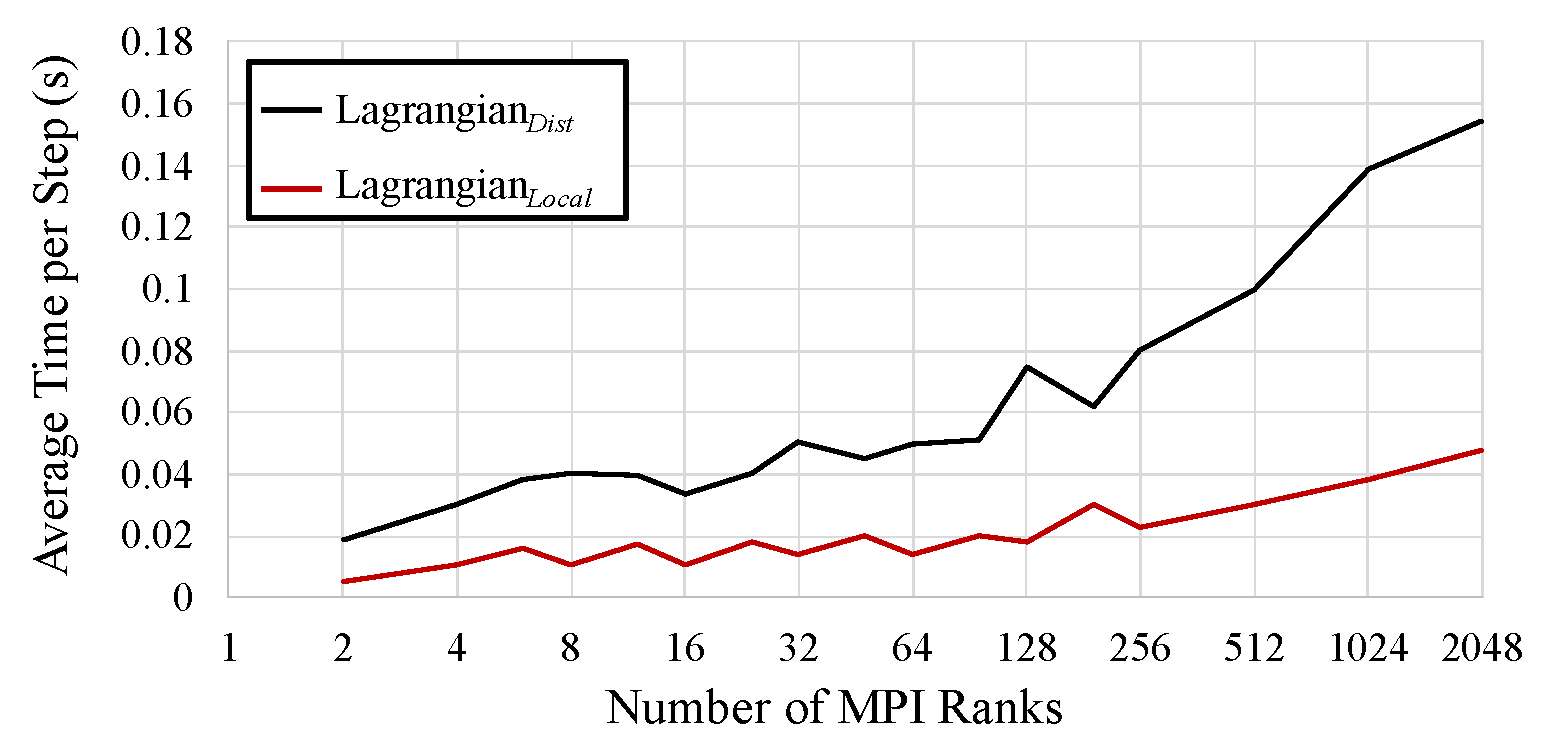
\includegraphics[width=0.9\linewidth]{Images/total_time.pdf}
\caption{Weak scaling study using in situ infrastructure to compute Lagrangian flow maps for the Cloverleaf3D data set.}
\label{fig:total_time}
\end{figure}

\begin{figure}[!b]
\vspace{-4mm}
\begin{subfigure}{0.495\linewidth}
\centering
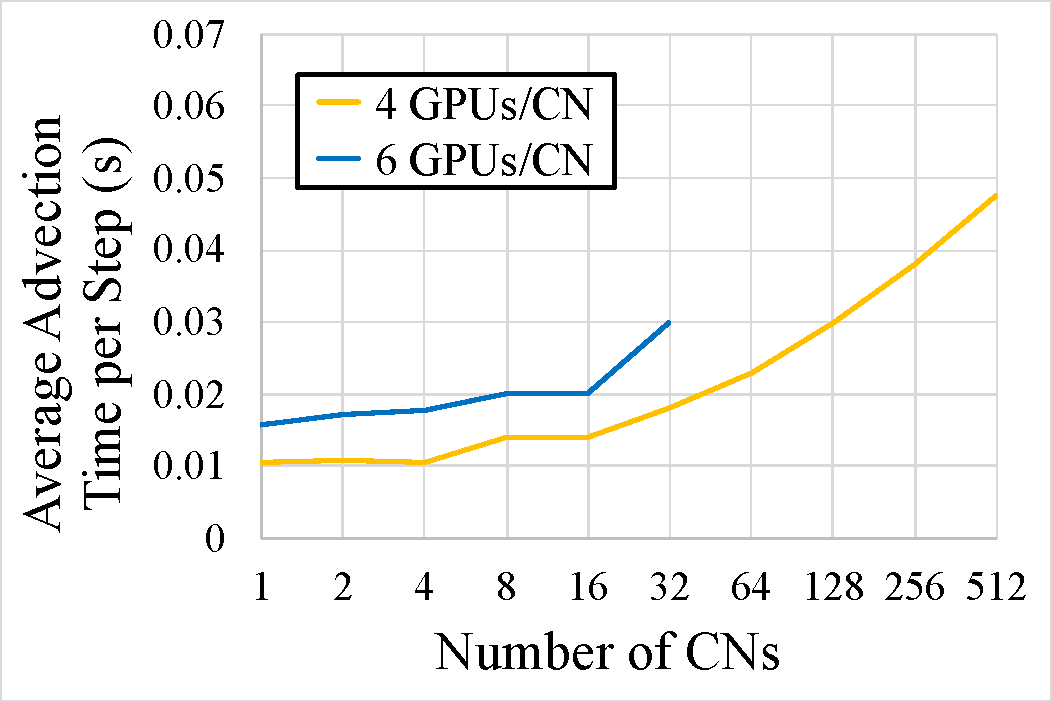
\includegraphics[width=\linewidth]{Images/advection_time2.pdf}
\vspace{-3mm}
\caption{Costs of particle advection.}
\label{fig:advection}
\end{subfigure}
\begin{subfigure}{0.495\linewidth}
\centering
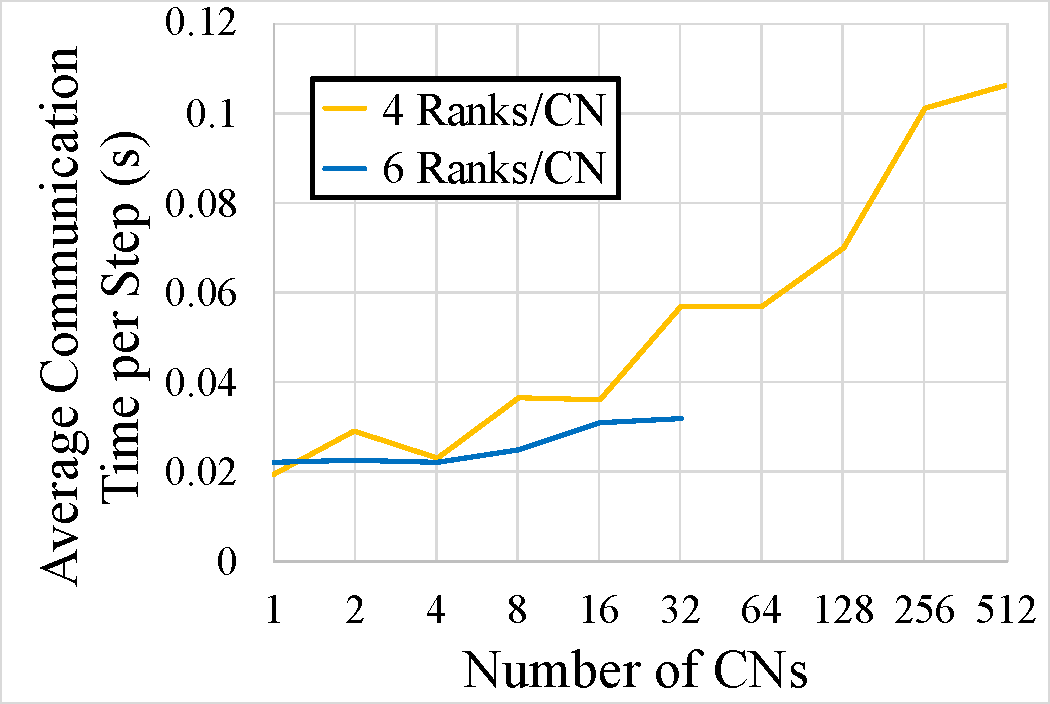
\includegraphics[width=\linewidth]{Images/communication_time2.pdf}
\vspace{-3mm}
\caption{Costs of communication.}
\label{fig:communication}
\end{subfigure}
\caption{\fix{Results for weak scaling the number of GPUs or ranks (4 or 6) per compute node. Lagrangian$_{Local}$ particle advection costs are plotted in~\ref{fig:advection} and Lagrangian$_{Dist}$ communication costs are in~\ref{fig:communication}. While particle advection performed better with fewer GPUs sharing memory on a single compute node~(\ref{fig:advection}), communication benefitted from MPI optimizations when more ranks execute on a single compute node~(\ref{fig:communication}).}} 
\label{fig:gpu_nodes}
\end{figure}


\textbf{Varying GPUs/Ranks per Compute Node.}
Since each CN on Summit has 6 GPUs a simulation can be configured in several ways.
%
In our tests, each rank has a dedicated GPU and operates on approximately the same number of particles.
%
Varying the number of ranks on each CN impacts both particle advection and communication costs.
%
Using data points from our weak scaling \textbf{Workflow1} study, we analyze these effects.
%

Figure~\ref{fig:advection} isolates the costs of particle advection per step of Lagrangian$_{Local}$.
%
Particle advection performs better with 4 GPUs per CN versus 6.
%
Use of shared memory by multiple GPUs on a single CN and saturation of the NVLink by the VTK-m particle advection kernel causes this effect.
%

Figure~\ref{fig:communication} shows the difference in communication costs per step for Lagrangian$_{Dist}$.
%
In contrast to the particle advection costs, the MPI communication cost shows a reduction when using 6 ranks versus 4 per CN. 
%
The data points using 4 ranks per CN show poor scalability as the number of CNs continues to increase.
%
On-node MPI communication optimizations contribute to better performance when grouping a larger number of MPI ranks on each CN, but the communication cost of inter-node remains high in comparison to intra-node and increases with number of CNs.

%
%Although these results inform computational performance, the specific configuration is determined by the simulation.
%

\textbf{Reconstruction Accuracy.}
We calculated the reconstruction accuracy for a subset of the Lagrangian$_{Local}$ weak scaling \textbf{Workflow1} configurations since it takes prohibitively long periods of time for the larger grid sizes on our single-node local machine.
%
Configurations terminated 2\%-5\% of particles and consequently stored 95\%-98\% of all initially seeded trajectories. 
%
We measured the accuracy of reconstructing the discarded trajectories only and present the results using violin plots in Figure~\ref{fig:clover_plot}.
%
As the simulation grid resolution increases, the grid cell size and particle advection step size decrease, while the total number of particles sampling the domain increases. 
%
Over 75\% of discarded trajectories have reconstruction error under 25\% of a GCS from the ground truth.
%
Further, this trend was observed across all the 8 test configurations we reconstructed. 

Reconstruction accuracy, however, is not constant across all storage intervals and demonstrates temporal patterns.
%
%
Figure~\ref{fig:clover_map} uses a heatmap for reconstruction accuracy across every interval of a Cloverleaf3D test. 
%
Measuring reconstruction accuracy for individual intervals could provide insight into the suitability to compute local Lagrangian flow maps versus incur communication costs to retain all particles trajectories.
%
%This concept can extend to consider spatial patterns as well. 

\begin{figure}[!t]
\vspace{-2mm}
\centering
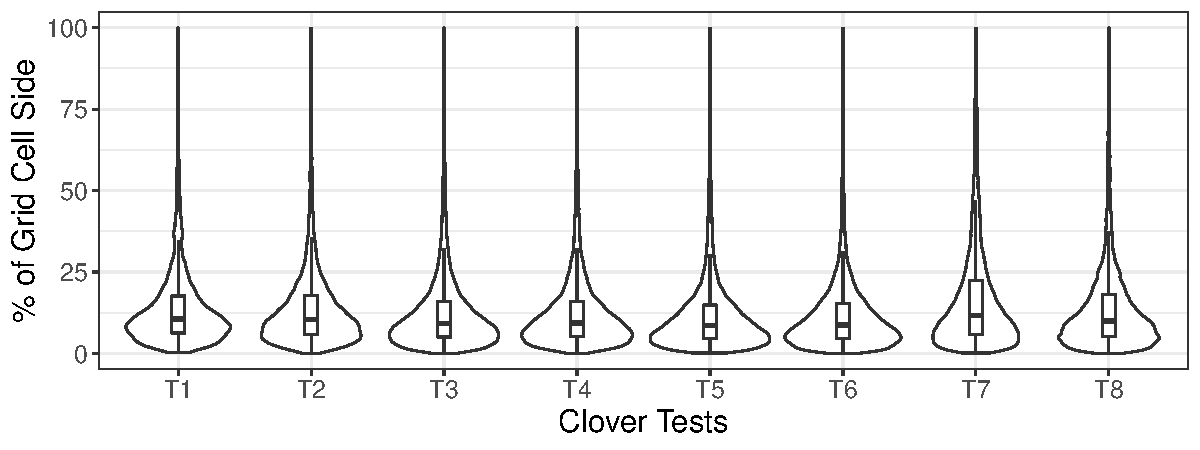
\includegraphics[width=\linewidth]{Images/Clover_Tests_1_8.pdf}
\caption{The distribution of the reconstruction error for eight Cloverleaf3D tests (labeled T1 through T8). The grid dimensions increase l-r from $81^{3}$ to $204^{3}$ over 500 cycles.}
\label{fig:clover_plot}
\vspace{-3mm}
\end{figure}

\begin{figure}[!t]
\centering
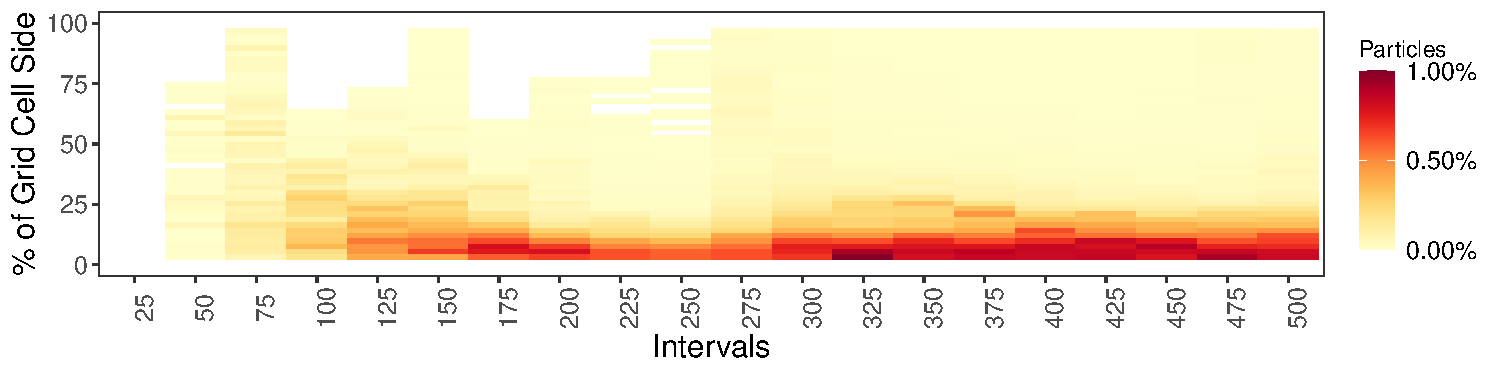
\includegraphics[width=\linewidth]{Images/Clover_Intervals_T8.pdf}
\caption{The Cloverleaf3D data set reconstruction error for all the intervals of a single test configuration~(T8).}
\vspace{-2mm}
\label{fig:clover_map}
\end{figure}



Overall, using Lagrangian$_{Local}$ with a storage interval of 25 cycles and 1:8 data reduction factor, the complete Lagrangian flow map can be reconstructed with high accuracy while providing speed-ups of 2x-4x for the Cloverleaf3D data set.

\textbf{Impact of Domain Decomposition.}
%
\begin{figure}[!t]
\centering
%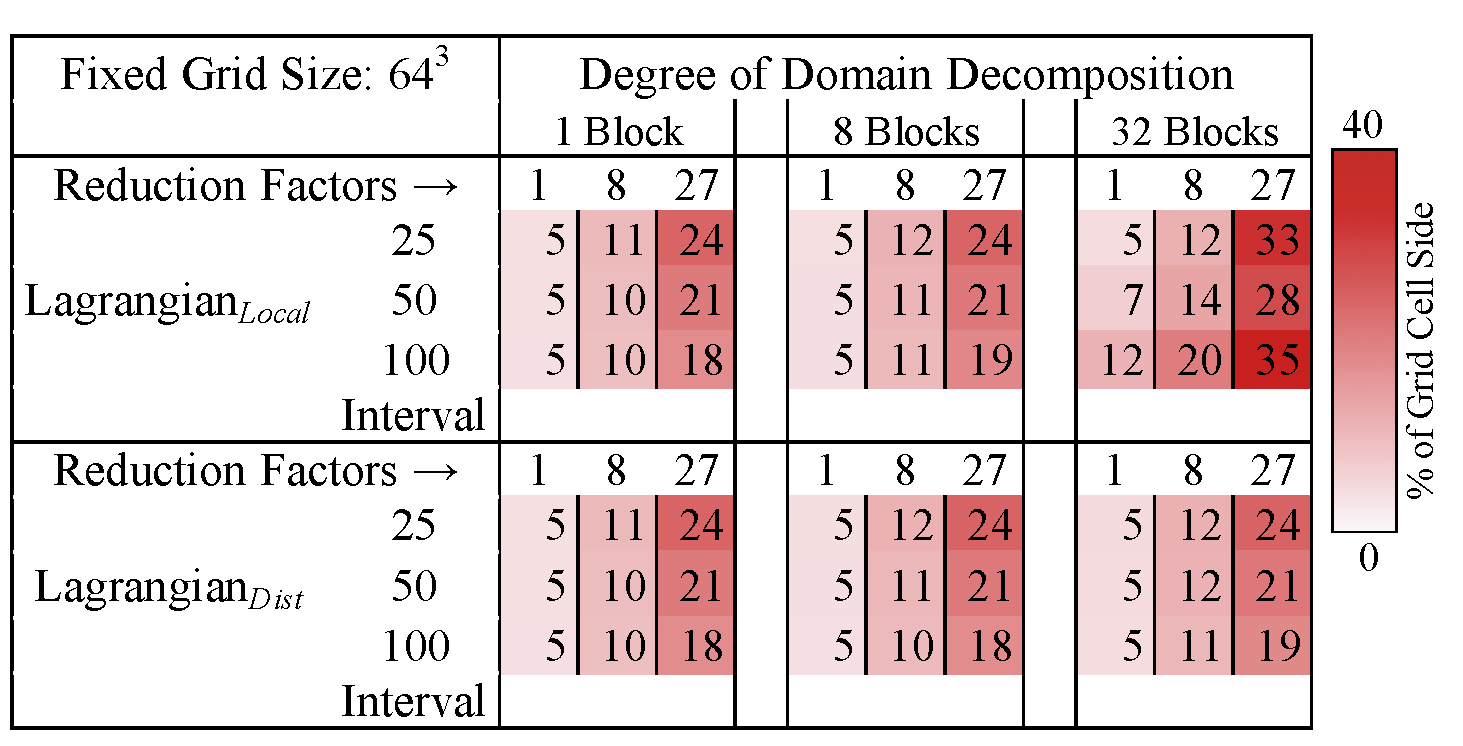
\includegraphics[width=\linewidth, trim={1.25cm 6.5cm 1.25cm 6.5cm}, clip]{Images/strongscaling.pdf}
%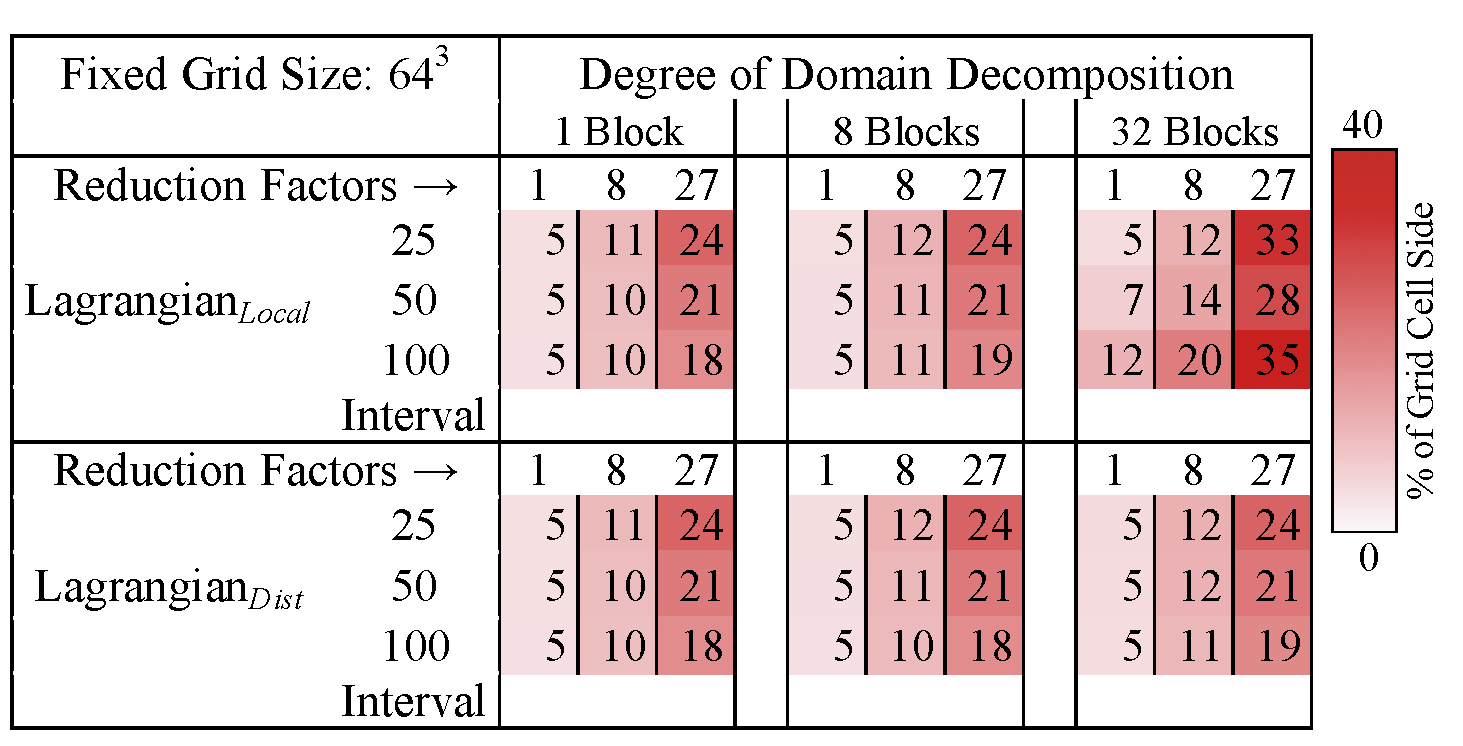
\includegraphics[width=\linewidth, trim={1.5cm, 16.8cm, 2cm, 1.8cm}, clip]{Images/strongscaling.pdf}
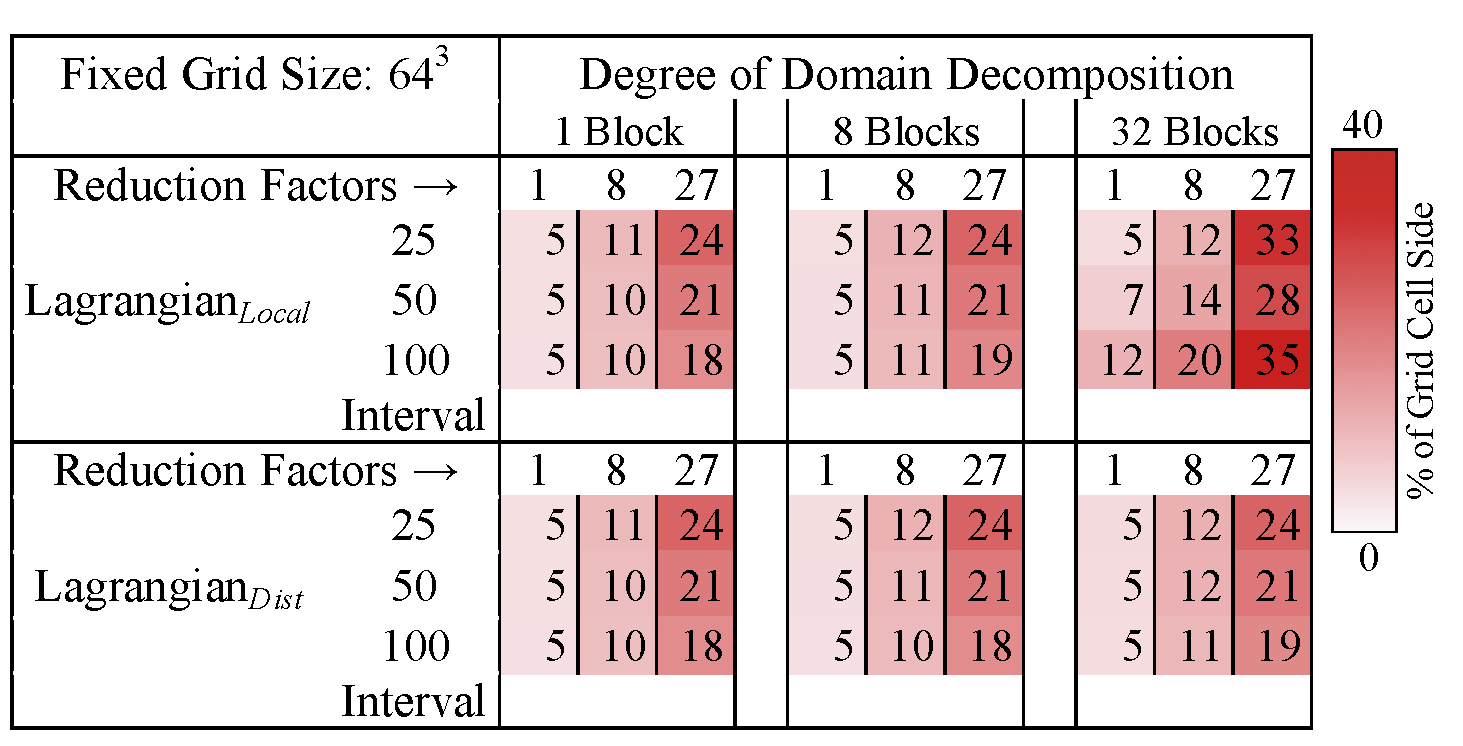
\includegraphics[width=0.95\linewidth]{Images/strongscaling.pdf}
\caption{Average error of new pathlines traced using Lagrangian$_{Dist}$ and Lagrangian$_{Local}$ for varying domain decomposition, storage interval, and data reduction factor. Here, a $64^{3}$ Cloverleaf3D data set defined over 800 cycles is used. Accuracy measurements are compared to the ground truth.} 
\vspace{-5mm}
\label{fig:strongscaling}
\end{figure}

%
Multiphysics HPC simulations typically have millions of grid points per rank and increase grid resolution as the number of ranks increases. 
%
To identify limitations, we evaluate Lagrangian$_{Local}$ in situations where this is not the case and consider the outcome when the number of processes operating over a fixed grid size increases.
%
%Although multiphysics HPC simulations typically have hundreds of thousands of grid points per data block, we evaluate Lagrangian$_{Local}$ in situations where this is not the case and the number of processes operating over a fixed grid increases .
%

Since the Lagrangian$_{Local}$ strategy is to discard trajectories exiting the rank-specific domain, this approach is susceptible to low resolution data blocks (i.e, sampling would use a small number of particles per rank) and longer storage intervals (i.e., integration times).
%
This \textbf{AE1} experiment measures the error of $1,000$ new pathlines generated for 800 cycles compared to the ground truth. 
%
Further, three parameter options are considered for domain decomposition, storage interval, and data reduction factor. 
%
Figure~\ref{fig:strongscaling} shows the pathline error when interpolating the flow maps generated by Lagrangian$_{Dist}$ and Lagrangian$_{Local}$. 
%
The accuracy of Lagrangian$_{Local}$ remains close to Lagrangian$_{Dist}$ until the domain decomposition is at its highest ($64^{3}$ grid decomposed across 32 ranks).
%
%
Although the overall accuracy of the interpolated pathlines is high (within a single GCS on average for all tests), both techniques lose some accuracy as the storage interval and data reduction factor increase, with Lagrangian$_{Local}$ performing worse under greater domain decomposition.
%
These results highlight the limitations of the Lagrangian$_{Local}$ technique as is.
%
%That said, we discuss approaches that could mitigate these limitations in Section~\ref{sec:discussion}.

\begingroup
\vspace{-2mm}
\begin{table}[!h]
\centering
\caption{Comparison of Lagrangian$_{Local}$ and the traditional approach, i.e., the Eulerian representation with temporal subsampling, for the Cloverleaf3D dataset. The error is the average percentage of grid cell side and is computed for 100,000 pathlines over 600 cycles. The unit for storage is GB.}
\resizebox{\columnwidth}{!}{%
\begin{tabular}{|c||c|c|c|c|}
\hline
Storage & \multicolumn{2}{c|}{Lagrangian$_{Local}$} & \multicolumn{2}{c|}{Eulerian} \\
Interval & Avg \% of GCS & Storage & Avg \% of GCS & Storage \\
\hline
20 & 18.8 & 34 & 115.4 & 267 \\
40 & 25.2 & 17 & 269.0 & 133 \\
60 & 37.5 & 12 & 424.8 & 95 \\
\hline
\end{tabular}
}
\label{clover_eul_table}
\end{table}
\endgroup

\textbf{Comparison to Traditional Approach.}
\textbf{AE2} compares Lagrangian$_{Local}$ to using an Eulerian representation with temporal subsampling.
%
Table~\ref{clover_eul_table} shows the results of \textbf{AE2}.
%
We considered three storage intervals: 20, 40, and 60.
%
We used 96 MPI ranks distributed across 16 CNs and a grid size of $586^3$.
%
Lagrangian$_{Local}$ used a data reduction of 1:8, whereas for the Eulerian technique we stored the full spatial resolution.
%
To compare accuracy, we reconstructed 100,000 randomly seeded pathlines for 600 cycles.
%
%
Overall, Lagrangian$_{Local}$ is increasingly accurate (6x to 11x) compared to the Eulerian approach as the interval size increases, but requires less data storage.
%
These results align with findings in prior works~\cite{agranovsky2014improved, sane2018revisiting} that compared the use of Lagrangian representations to the traditional approach under sparse temporal settings.

\begin{figure}[h]
\centering
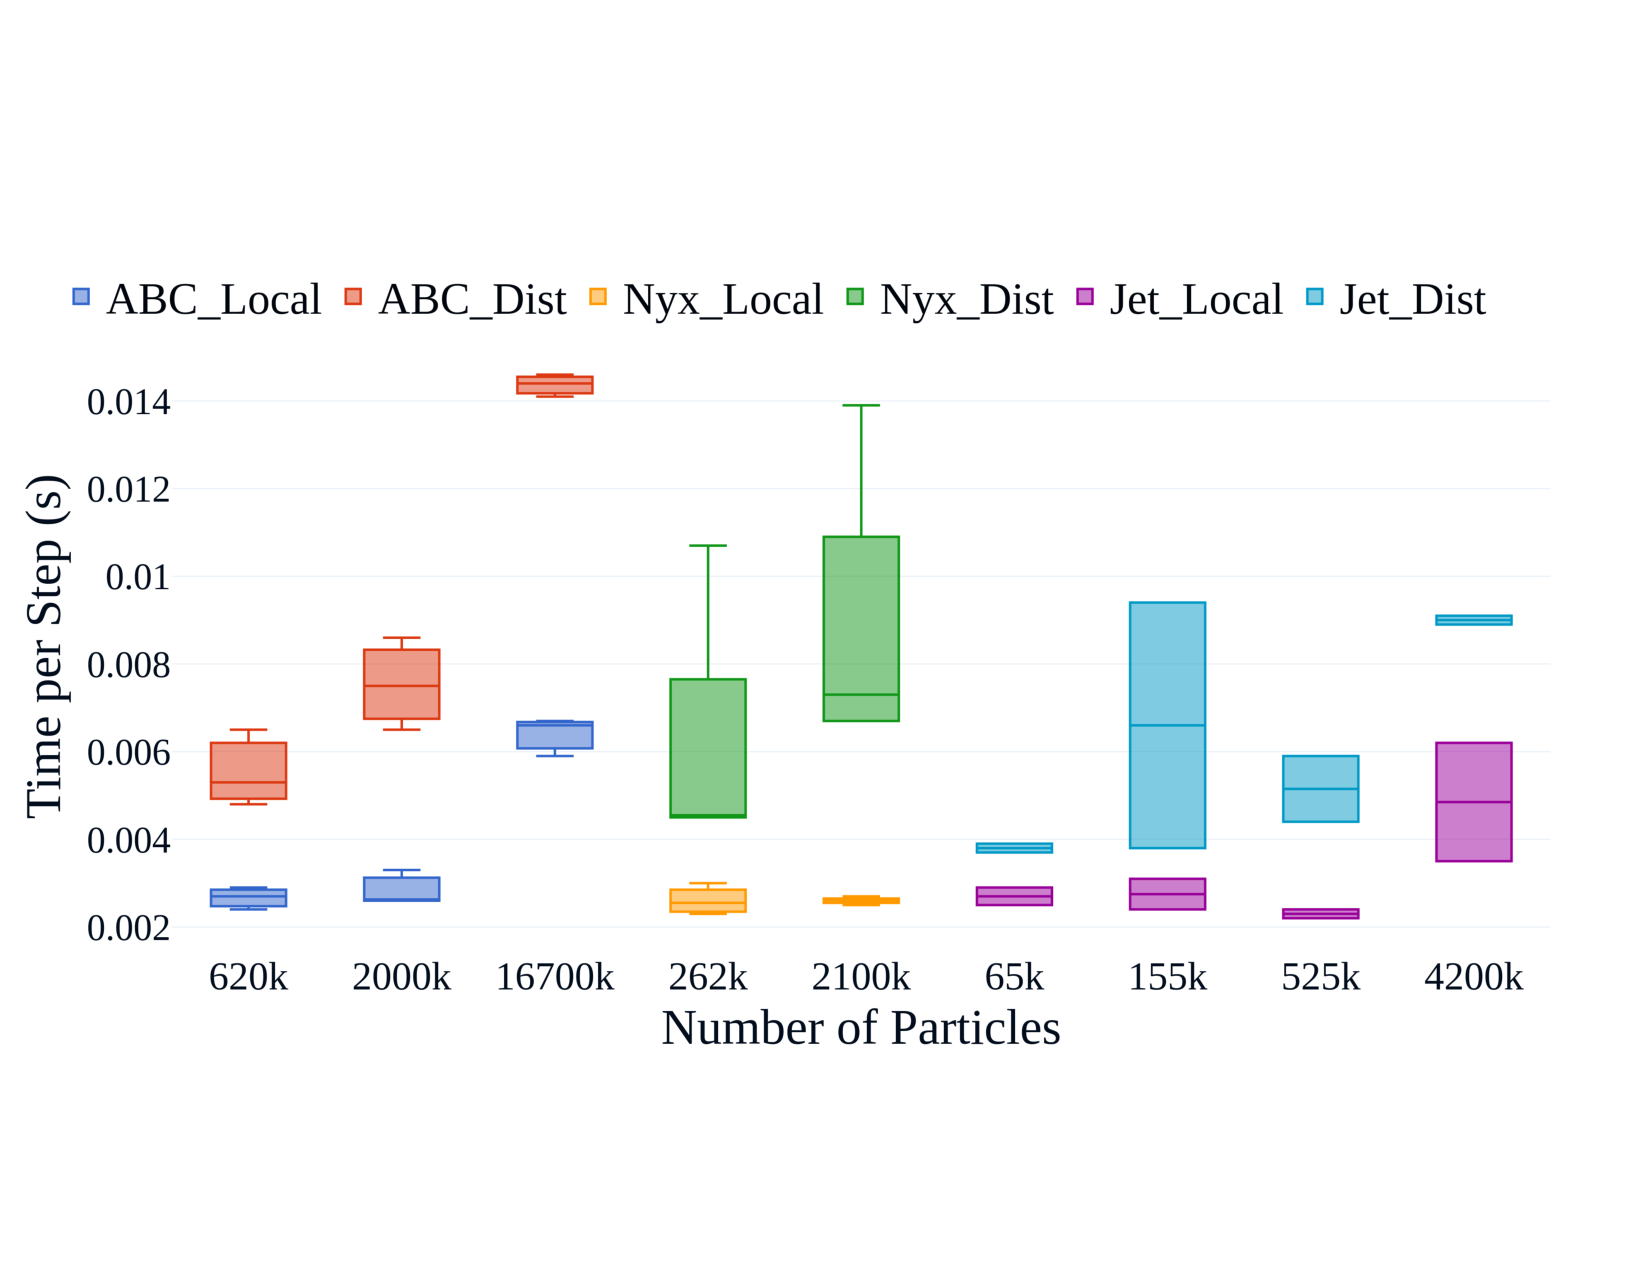
\includegraphics[width=\linewidth, trim={0.45cm 3.5cm 2cm 4.5cm}, clip]{Images/dataset_timings4.pdf}
\caption{Execution time per step of Lagrangian$_{Dist}$ and Lagrangian$_{Local}$ grouped by data set and ordered by the number of particles for \textbf{Phase-II} experiments.}
\label{fig:dataset_timings}
\end{figure}

\subsection{ABC Flow}
\label{sec:abc}

Table~\ref{abc_tab} lists all the ABC \textbf{Workflow2} test configurations, Figure~\ref{fig:dataset_timings} contains computation costs, and Figure~\ref{fig:abc_plot} shows the distribution of trajectory reconstruction error for each test.
%
\begingroup
\begin{table}[h]
\centering
\scalebox{0.9}{
%\resizebox{\columnwidth}{!}{
\begin{tabular}{|c||c|c|c|c|c|c|}
\hline
\textbf{Test} & \textbf{Interval} & \textbf{Reduction} & \textbf{Particles} & \textbf{Stored} & \textbf{Discarded} \\
\hline
T1 & 25 & \multirow{3}{*}{1:1} & \multirow{3}{*}{16700k} & 96.9\% & 3.1\% \\
T2 & 50 & & & 94.3\% & 5.7\%  \\
T3 & 100 & & & 89.7\% & 10.3\% \\
\hline
T4 & 25 & \multirow{3}{*}{1:8} & \multirow{3}{*}{2098k} & 97.7\% & 2.3\% \\
T5 & 50 & & & 95.2\% & 4.8\% \\
T6 & 100 & & & 90.6\% & 9.4\% \\
\hline
T7 & 25 & \multirow{3}{*}{1:27} & \multirow{3}{*}{621k} & 98.6\% & 1.4\% \\
T8 & 50 & & & 95.9\% & 4.1\% \\
T9 & 100 & & & 91.8\% & 8.2\% \\
\hline
\end{tabular}
}
\caption{\fix{Specifications for 9 ABC tests. In most cases, over 90\% of the complete flow map was stored.}}
\vspace{-2mm}
\label{abc_tab}
\end{table}
\endgroup

\begin{figure}[!b]
\vspace{-4mm}
\centering
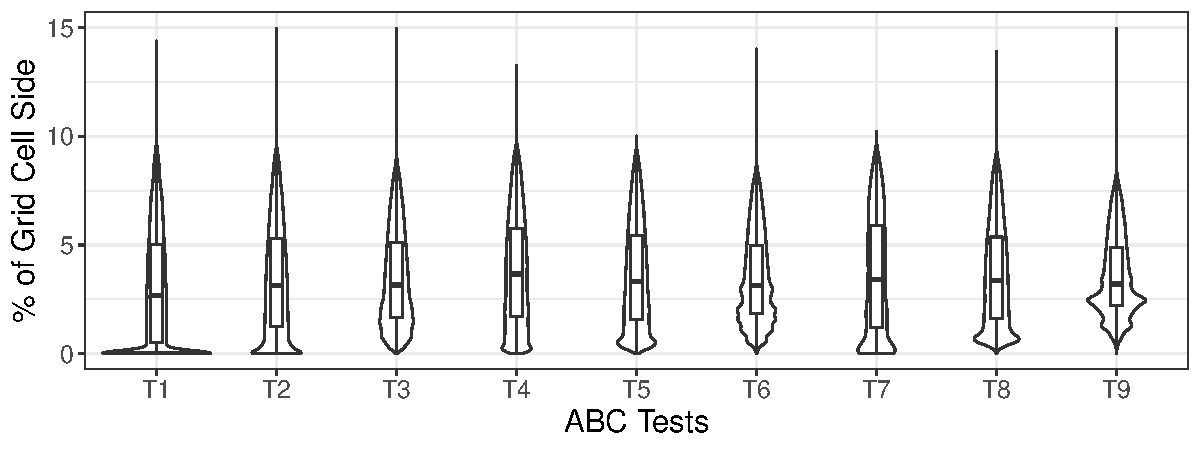
\includegraphics[width=\linewidth]{Images/ABC_Tests.pdf}
\caption{\fix{Violin plots of reconstruction error for the ABC data set tests labeled T1-T9. The plots show the error remained within a consistent range across tests, with only small increases as the data reduction factor and storage interval increase.}}
%\caption{Distribution of reconstruction error for ABC tests.}
\vspace{-2mm}
\label{fig:abc_plot}
\end{figure}


\textbf{Execution Time.} Using 64 MPI ranks, each with 1 GPU, across 16 CNs, Lagrangian$_{Dist}$ requires up to 2.8x more execution time as Lagrangian$_{Local}$.
%
Figure~\ref{fig:dataset_timings} shows particle advection and communication costs are directly proportional to the particle count.
%
Further, particle advection for up to 2M particles, i.e., 32k particles per GPU, can be performed in under 0.004 seconds per step for all data sets.
%
\begin{figure}[!ht]
\begin{subfigure}{\linewidth}
\centering
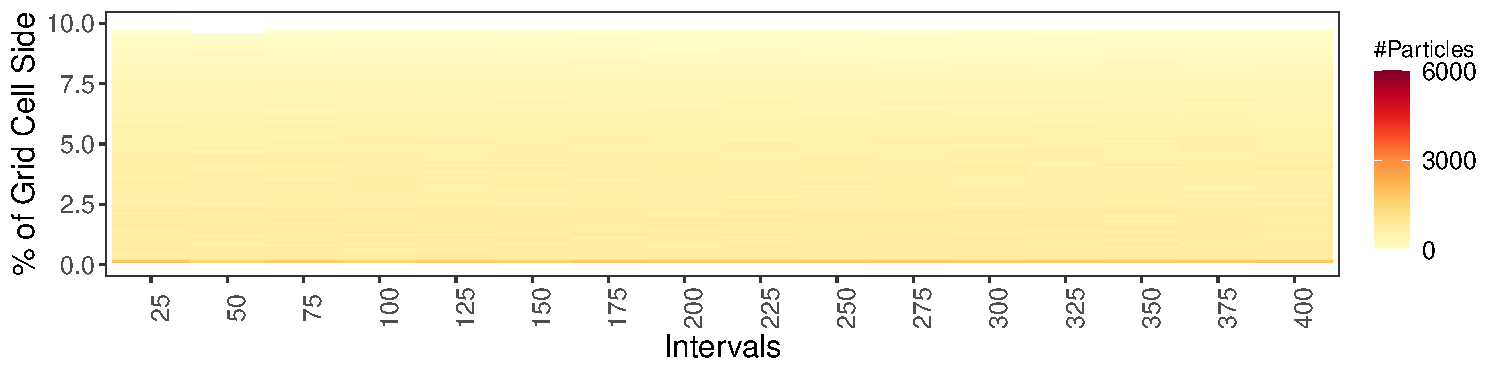
\includegraphics[width=\linewidth]{Images/ABC_Intervals_T4.pdf}
\vspace{-5mm}
\caption{T4, storage interval = 25 cycles}
\label{fig:abc_4}
\end{subfigure}
%\begin{subfigure}{\linewidth}
%\centering
%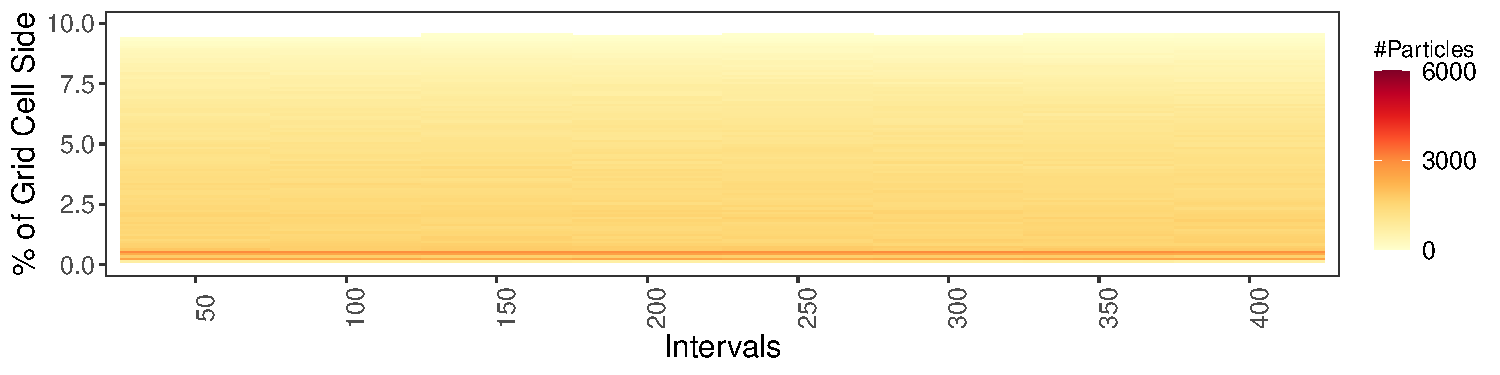
\includegraphics[width=\linewidth]{Images/ABC_Intervals_T5.pdf}
%\caption{T5, storage interval = 50 cycles}
%\label{fig:abc_5}
%\end{subfigure}
\begin{subfigure}{\linewidth}
\centering
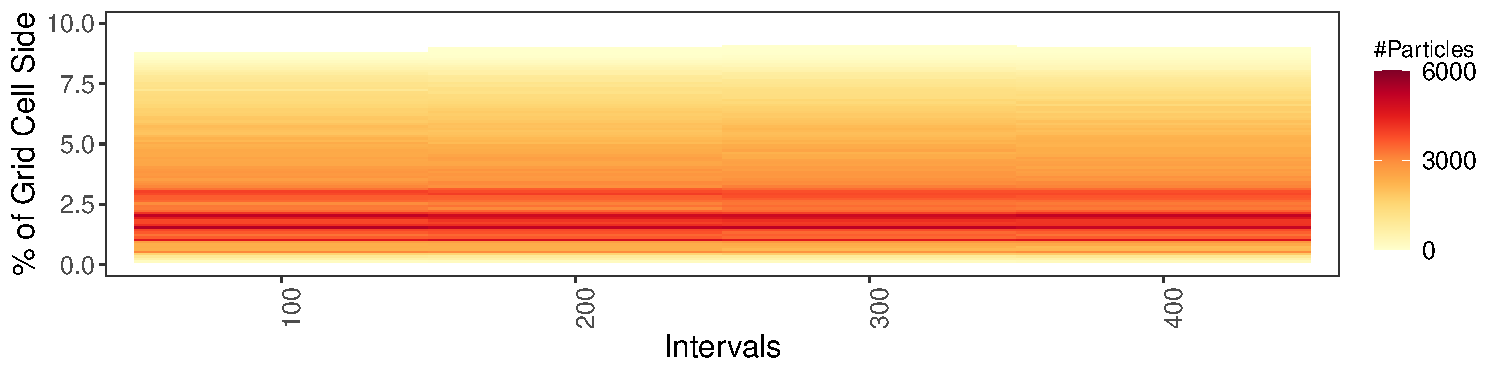
\includegraphics[width=\linewidth]{Images/ABC_Intervals_T6.pdf}
\vspace{-5mm}
\caption{T6, storage interval = 100 cycles}
\label{fig:abc_6}
\end{subfigure}
\caption{\fix{Heatmap of reconstruction error for the ABC data set as a function of interval. These plots show that the majority of reconstructed trajectories are within a grid cell side of the ground truth, despite the larger of number of discarded particles resulting from the larger storage interval~(\ref{fig:abc_6}).}}
%\caption{\fix{For the ABC data set, although increasing the storage interval resulted in a larger number of discarded particles, the majority of reconstructed trajectories are within a grid cell side of the ground truth.}} 
%\caption{ABC data set tests showing impact of variation in storage interval on the distribution of reconstruction error.}
\vspace{-5mm}
\label{fig:abc_map}
\end{figure}


\textbf{Reconstruction Accuracy.} Figure~\ref{fig:abc_plot} indicates the ABC data set shows shifts in reconstruction error distribution when varying the storage intervals and sampling resolution while remaining within similar ranges.
%
Overall, the discarded trajectories from the ABC data set Lagrangian flow map can be reconstructed very accurately, with trajectories interpolated to the same grid cell as the ground truth.
%
Specifically, reconstructions are under 10\% of a GCS away from the ground truth.
%

\textbf{Impact of Varying Storage Interval.} Figure~\ref{fig:abc_map} shows heatmaps of the reconstruction error across all intervals for tests T4, T5, and T6.
%
Comparing the heatmaps, the effect of increasing the storage interval is a larger number of particles are terminated in a single interval. 
%
Further, the reconstruction error distribution matches the violin plots of T4, T5, and T6 in Figure~\ref{fig:abc_plot}. 
%
Even for longer storage intervals, the error remains small, and discarded trajectories are reconstructed with high accuracy for the ABC data set.

\subsection{Nyx Cosmology}
\label{sec:nyx}
Table~\ref{nyx_tab} lists all the Nyx \textbf{Workflow2} test configurations, Figure~\ref{fig:dataset_timings} contains computation costs, and Figure~\ref{fig:nyx_plot} shows the distribution of trajectory reconstruction error for each test.
%
\begingroup
\begin{table}[!h]
\centering
\scalebox{0.9}{
%\resizebox{\columnwidth}{!}{%
\begin{tabular}{|c||c|c|c|c|c|c|}
\hline
\textbf{Test} & \textbf{Interval} & \textbf{Reduction} & \textbf{Particles} & \textbf{Stored} & \textbf{Discarded} \\
\hline
T1 & 10 & \multirow{4}{*}{1:1} & \multirow{4}{*}{2097k} & 96\% & 4\% \\
T2 & 20 & & & 92.1\% & 7.9\% \\
T3 & 40 & & & 85.7\% & 14.3\%  \\
T4 & 50 & & & 83\% & 17\% \\
\hline
T5 & 10 & \multirow{4}{*}{1:8} & \multirow{4}{*}{262k} & 97.4\% & 2.6\% \\
T6 & 20 & & & 93.7\% & 6.3\% \\
T7 & 40 & & & 88.2\% & 11.8\% \\
T8 & 50 & & & 85.8\% & 14.2\% \\
\hline
\end{tabular}
}
%}
\caption{\fix{Specifications for 8 Nyx tests. We observed the largest number of discarded particles for this data set.}}
\vspace{-2mm}
\label{nyx_tab}
\end{table}
\endgroup


\textbf{Execution Time.} Across our 8 tests using the Nyx data set, Lagrangian$_{Local}$ computed a flow map up to 5.2x faster than the corresponding Lagrangian$_{Dist}$ flow map.
%
Additionally, Figure~\ref{fig:dataset_timings} shows the standard deviation is greater for the Lagrangian$_{Dist}$ tests and is caused by the larger number of particles exchanges between ranks for this data set.
%

\textbf{Reconstruction Accuracy.} As a consequence of a large number of particles being discarded by Lagrangian$_{Local}$, the accuracy of reconstruction is impacted by the longer storage intervals.
%
Although 7 of 8 tests show up to the third quartile reconstructing under 100\% of a GCS, the number of instances with a higher reconstruction error increases with the storage interval.
%
However, for shorter storage interval lengths (10, 20), the reconstruction quality is high for both data reduction factors considered. 
%
Lastly, Figure~\ref{fig:nyx_map} uses a heatmap to show the distribution of error across every interval. 
% of a Nyx configuration.

\begin{figure}[!h]
\centering
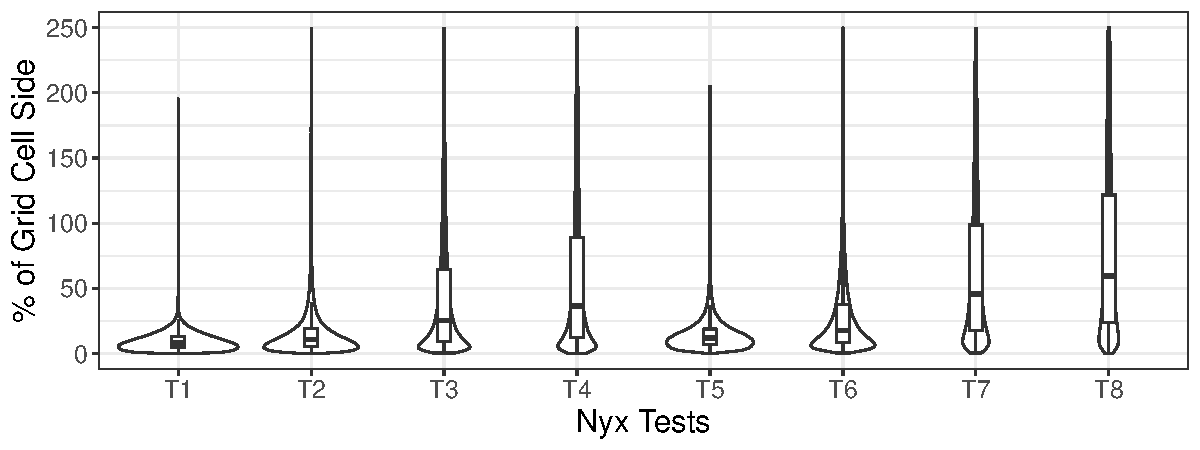
\includegraphics[width=\linewidth]{Images/Nyx_Tests.pdf}
\caption{Distribution of the reconstruction error for Nyx tests.}
\label{fig:nyx_plot}
\end{figure}

\begin{figure}[!h]
\centering
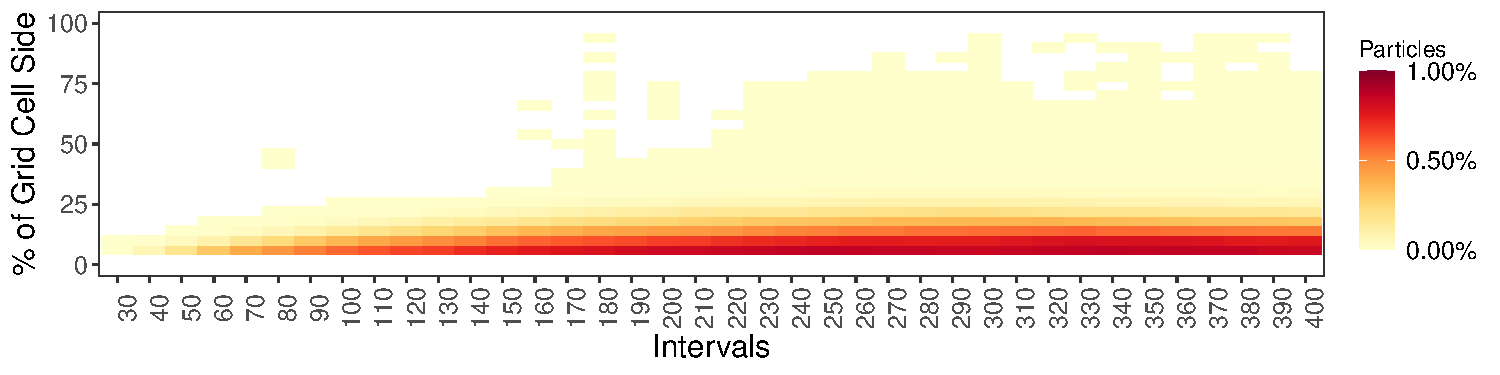
\includegraphics[width=0.95\linewidth]{Images/Nyx_Intervals_T1.pdf}
\caption{The Nyx data set reconstruction error for all the intervals of a single test configuration~(T1).}
\label{fig:nyx_map}
\end{figure}


\subsection{Jet Flow}
\label{sec:jet}
Table~\ref{jet_tab} lists all the Jet \textbf{Workflow2} test configurations, Figure~\ref{fig:dataset_timings} contains computation costs, and Figure~\ref{fig:jet_plot} shows the distribution of trajectory reconstruction error for each test.
%
\begingroup
\begin{table}[!b]
\vspace{-2mm}
\centering
\caption{\fix{Specifications for 8 Jet tests. In most cases, under 2\% of particle trajectories are discarded. Accurate reconstruction of these trajectories~(see Figure~\ref{fig:jet_plot}) was dependent on the absolute number of stored particles.}}
\scalebox{0.9}{
%\resizebox{\columnwidth}{!}{%
\begin{tabular}{|c||c|c|c|c|c|c|}
\hline
\textbf{Test} & \textbf{Interval} & \textbf{Reduction} & \textbf{Particles} & \textbf{Stored} & \textbf{Discarded} \\
\hline
T1 & 5 & \multirow{2}{*}{1:1} & \multirow{2}{*}{4194k} & 99.4\% & 0.6\% \\
T2 & 10 & & & 97.9\% & 2.1\% \\
\hline
T3 & 5 & \multirow{2}{*}{1:8} & \multirow{2}{*}{524k} & 99.6\% & 0.4\% \\
T4 & 10 & & & 98.9\% & 1.1\% \\
\hline
T5 & 5 & \multirow{2}{*}{1:27} & \multirow{2}{*}{155k} & 99.7\% & 0.3\% \\
T6 & 10 & & & 99.1\% & 0.9\% \\
\hline
T7 & 5 & \multirow{2}{*}{1:64} & \multirow{2}{*}{65k} & 99.8\% & 0.2\% \\
T8 & 10 & & & 99.3\% & 0.7\% \\
\hline
\end{tabular}
}
\vspace{-2mm}
\label{jet_tab}
\end{table}
\endgroup


\textbf{Execution Time.} For the Jet data set, Lagrangian$_{Local}$ computed a flow map up to 3.9x faster than the corresponding Lagrangian$_{Dist}$ flow map.
%
For this data set, we considered shorter storage intervals, and thus a smaller percentage of particles required particle exchange to continue trajectory integration.
%
However, Figure~\ref{fig:dataset_timings} shows the variability in the cost of communication as it is susceptible to network usage and bandwidth contention.
%

\textbf{Reconstruction Accuracy.} The Jet data set presents an adversarial case for our proposed optimization of computing local flow maps.
%
The data set contains regions with high velocity magnitude.
%
Across the range of configurations in Figure~\ref{fig:jet_plot}, both the storage interval and the data reduction factor impact the reconstruction accuracy.
%
Further investigation into the distribution of T2 revealed that the longer storage interval resulted in several particles terminating in easy-to-reconstruct areas of the domain at the start of the simulation (most other configurations show particle termination only after cycle 30).
%
%
The sparser sampling for other configurations with the same storage interval misses this effect.
%
Further, as the number of samples used reduces, the reconstruction of discarded trajectories can be multiple cells away from the ground truth.
%
For example, T8 using 1:64 data reduction factor and a storage interval of 10, has a mean reconstruction of 150% of GCS.
\begin{figure}[!b]
\centering
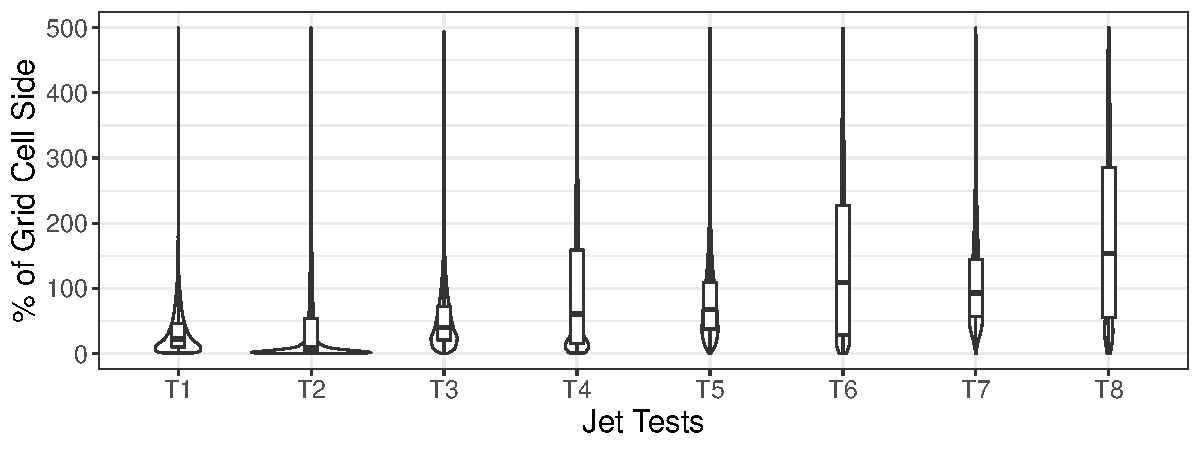
\includegraphics[width=\linewidth]{Images/Jet_Tests.pdf}
\caption{\fix{Violin plots of reconstruction error for the Jet data set tests labeled T1-T8. The plots show that error increased significantly with increased data reduction factor and storage interval. Reconstruction error was low only when no data reduction~(1:1) was used~(T1, T2).}}
%\caption{\fix{As in Figure~\ref{fig:nyx_plot}, reconstruction error for the Jet data set increased significantly with increased data reduction factor and storage interval. We found reconstruction accuracy within a grid cell side for most particles only when no data reduction~(1:1) was used~(T1, T2).}}
%\caption{Distribution of the reconstruction error for Jet tests.}
\vspace{-2mm}
\label{fig:jet_plot}
\end{figure}

\begin{figure}[!b]
\begin{subfigure}{\linewidth}
\centering
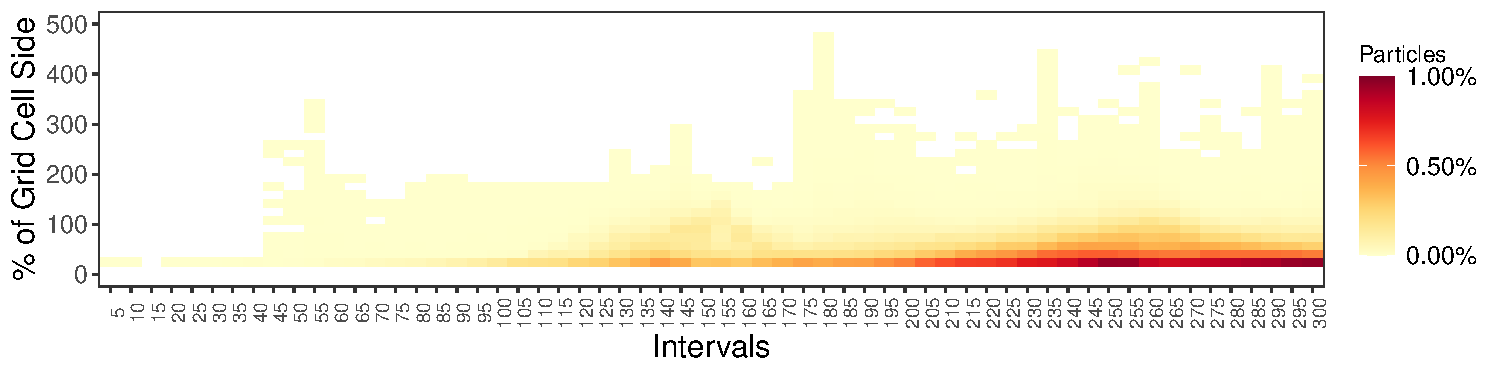
\includegraphics[width=\linewidth]{Images/Jet_Intervals_T1_Percent.pdf}
\caption{T1, 1:1}
\label{fig:jet_1}
\end{subfigure}
\begin{subfigure}{\linewidth}
\centering
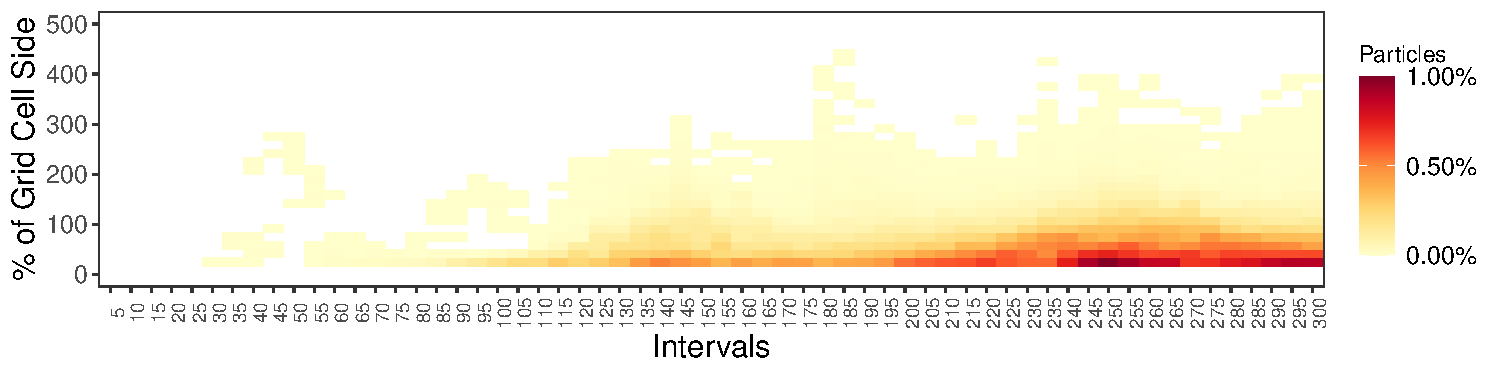
\includegraphics[width=\linewidth]{Images/Jet_Intervals_T3_Percent.pdf}
\caption{T3, 1:8}
\label{fig:jet_3}
\end{subfigure}
\begin{subfigure}{\linewidth}
\centering
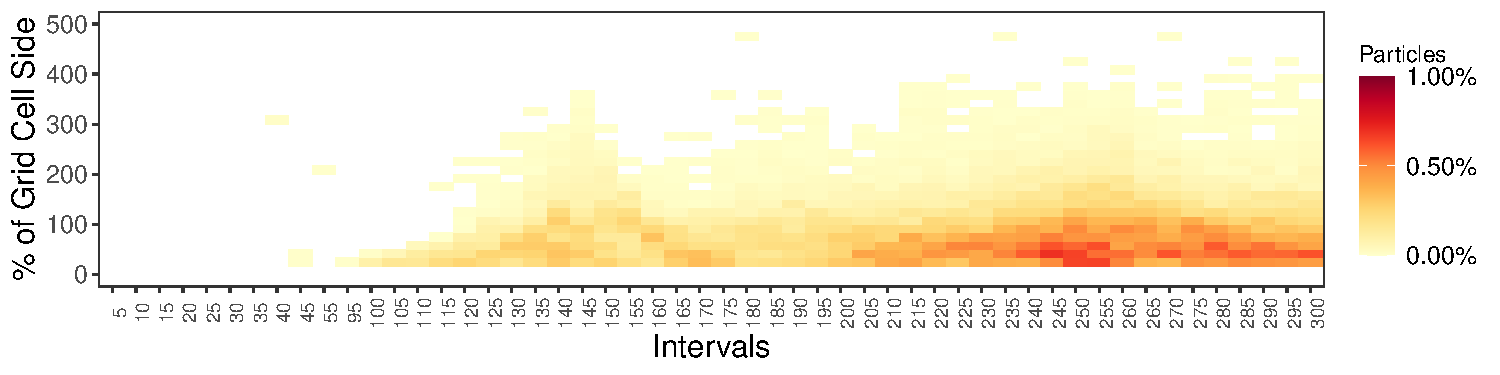
\includegraphics[width=\linewidth]{Images/Jet_Intervals_T5_Percent.pdf}
\caption{T5, 1:27}
\label{fig:jet_5}
\end{subfigure}
\begin{subfigure}{\linewidth}
\centering
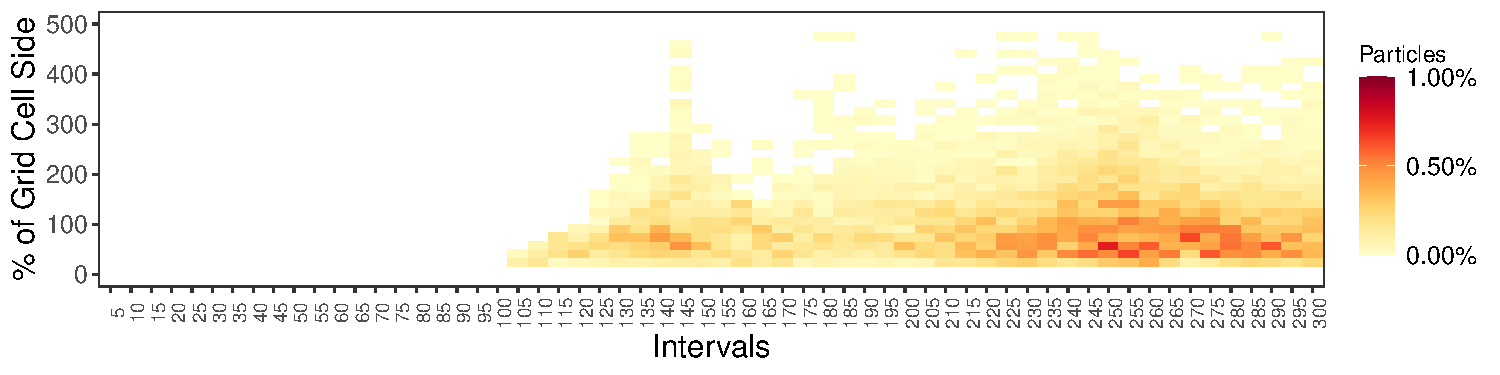
\includegraphics[width=\linewidth]{Images/Jet_Intervals_T7_Percent.pdf}
\caption{T7, 1:64}
\label{fig:jet_7}
\end{subfigure}
\caption{Jet tests showing the impact of variation in the data reduction factor on the distribution of reconstruction error.}
\label{fig:jet_map}
\end{figure}


\textbf{Impact of Varying Data Reduction Factor.} Figure~\ref{fig:jet_map} shows heatmaps comparing the distribution of reconstruction error across every interval.
%
Based on the distribution of error, the reconstruction accuracy is high when a 1:1 data reduction factor is used, and reduces in accuracy with fewer samples.
%
%
%
%Overall, based on the distribution of reconstruction accuracy, the probability of accurate reconstruction increases with more samples.

